\begin{figure}[tbp]
\begin{center}
\includegraphics[width=0.48\textwidth]{figure/cl_correlation_z1_z2.eps}
\end{center}
\vspace{-0.7cm}
\caption{The cross correlation r between real kSZ $P_{\Theta_{kSZ}}$ 
and reconstructed kSZ $P_{\hat \Theta_{kSZ}}$.
}
\label{fig:r}
\end{figure}
\label{ssec:tide}
The cross correlation between $v_z$ and $\hat v_z^{tide}$ are demonstrated in Fig.\ref{fig:v}. 
Important modes for velocity fields(redline of Fig.\ref{fig:k3p}) are well extracted with correlation greater than $0.7$. 
The reconstruction on $k_\parallel$ direction is better than on $k_\perp$ direction.
This is because tidal reconstruction relies heavily on large $k$ modes, 
yet lots of large $k_\perp$ modes, whose $k_\parallel$ is small, are lost in the foregrounds. 
There is degrading performance of tidal reconstruction on $z=2$ compared to $z=1$, 
which mainly results from the stricter cutoff $k_c=0.32$ h/Mpc compared to $k_c=0.5$ h/Mpc.

In Fig.\ref{fig:r}, 
we demonstrate the correlation r between the reconstructed kSZ signal $\hat \Theta_{tide}$ and original kSZ signal $\Theta$. 

It is important to see:
For $z=1$, there are significant improvement on the cross-correlation after tidal reconstruction, especially below $\ell \sim 2000$; 
for $z=2$, the cross-correlation is improved for $\ell \lesssim 800$. 
Combining noise filtered fields and tidal reconstructed fields, we shall have good cross-correlation for $\ell  \sim 50-5000$, 
with the assumed level of foregrounds and noises on small scales.

%In all, for both redshift, with the non-ideal foregrounds and resolutions we assume, 
%we are able to obtain a correlation $r \gtrsim 0.5$ for $\ell \sim 50-5000$ between 21 cm density field and kSZ signals.

